% LEGACY DOCUMENT (historical seminar talk wave 17)
% Current status: See RESEARCH_STATUS.md and TECH_TREE.md for canonical assessment.
% δ_CP prediction is WITHDRAWN (>5σ excluded by NuFIT-6.0 + T2K+NOvA 2025).
% See PREDICTIONS_PREREGISTERED.md for canonical up-to-date assessment.

\documentclass[aspectratio=169,11pt]{beamer}
\usetheme{default}
\usecolortheme{seahorse}

\usepackage{amsmath,amssymb,amsthm}
\usepackage{booktabs}
\usepackage{graphicx}
\usepackage{tikz}
\usepackage{slashed}

\newcommand{\ph}{\varphi}
\newcommand{\Dirac}{\slashed{D}}
\newcommand{\tr}{\operatorname{tr}}

\title{Trinity S$^3$AI}
\subtitle{An Active Boundary-Mapping Research Program in Geometric Unification}
\date{May 2026}
\author{Trinity S$^3$AI Research Collective}
\institute{\url{https://github.com/gHashTag/trinity-s3ai}}

\begin{document}

% ============================================================
\begin{frame}{Title}
  \titlepage
  \vfill
  \begin{center}
    \small\textit{``What H$_4$/600-cell can and cannot do for the Standard Model''}
  \end{center}
\note{Welcome the audience. Spoiler: answer is NO. Trinity S³AI tests if SM can be derived from H₄ geometry. Journey reveals interesting structures.}
\end{frame}

% ============================================================
\begin{frame}{Motivation: Why H$_4$/600-cell?}
  \begin{columns}
    \begin{column}{0.55\textwidth}
      \begin{itemize}
        \item H$_4$ is the largest finite Coxeter group in 4D: $|W(\text{H}_4)| = 14\,400$
        \item 600-cell has 120 vertices = binary icosahedral group $2I \subset SU(2)$
        \item Golden ratio $\ph$ appears in coordinates: $\tfrac12(0, \pm\ph^{-1}, \pm 1, \pm\ph)$
        \item McKay correspondence: $2I \leftrightarrow E_8$
        \item Hope: finite spectral triple on $2I$ $\to$ SM algebra $\mathbb{C}\oplus\mathbb{H}\oplus M_3(\mathbb{C})$
      \end{itemize}
    \end{column}
    \begin{column}{0.4\textwidth}
      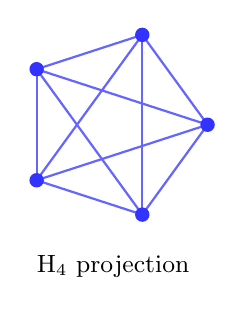
\begin{tikzpicture}[scale=1.2]
        \foreach \i in {0,72,...,288} {
          \draw[thick,blue!60] (\i:1) -- (\i+72:1);
          \draw[thick,blue!60] (\i:1) -- (\i+144:1);
        }
        \foreach \i in {0,72,...,288} {
          \filldraw[blue!80] (\i:1) circle (2pt);
        }
        \node at (0,-1.5) {\small H$_4$ projection};
      \end{tikzpicture}
    \end{column}
  \end{columns}
\note{H₄ = 14400 elements. 600-cell = 120 vertices = binary icosahedral group 2I ⊂ SU(2). McKay → E₈. Hope: finite spectral triple → SM algebra.}
\end{frame}

% ============================================================
\begin{frame}{Mathematical Framework: Discrete Dirac}
  \begin{itemize}
    \item Hilbert space: $\mathcal{H} = \mathbb{C}^{120} \otimes \mathbb{C}^4$ (vertices $\times$ spinors) = 480-dim
    \item Dirac operator: $(D\psi)_i = \sum_{j \sim i} \langle i j \rangle \cdot \gamma(\overrightarrow{ij})\, \psi_j$
    \item $D$ is Hermitian, chirally symmetric: $\{D, \gamma^5\} = 0$
    \item Spectrum: 240 positive + 240 negative eigenvalues, no zero modes
    \item Verified numerically (scipy, $480\times480$) and in Coq (\texttt{DiracOperator.v})
  \end{itemize}
  \vfill
  \begin{center}
    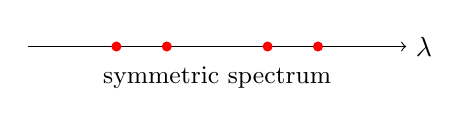
\begin{tikzpicture}[scale=0.8]
      \draw[->] (-3,0) -- (3,0) node[right] {$\lambda$};
      \foreach \x in {-2,-1,1,2} {
        \draw[red,fill=red] (\x*0.8,0) circle (2pt);
      }
      \node at (0,-0.5) {\small symmetric spectrum};
    \end{tikzpicture}
  \end{center}
\note{Hilbert space 480-dim (120×4). D is Hermitian, chirally symmetric. Spectrum: 240+ / 240−, no zero modes. Verified in SciPy and Coq (DiracOperator.v).}
\end{frame}

% ============================================================
\begin{frame}{KO-dimension: A Genuine Positive Result}
  \begin{itemize}
    \item Real structure $J$ = quaternionic conjugation
    \item Signs computed: $J^2 = +1$, $JD = +DJ$, $J\Gamma = +\Gamma J$ $\to$ $(+,+,+)$
    \item This sign triple is compatible with \textbf{KO-dim $6 \pmod 8$}
    \item KO-dim 6 is exactly what the Connes--Chamseddine SM requires
    \item \textbf{Caveat:} $(+,+,+)$ also fits KO-dim 0; distinction needs off-diagonal $J$ (admitted as structural axiom)
  \end{itemize}
  \vfill
  \begin{center}
    \begin{tabular}{cccc}
      \toprule
      KO-dim & $J^2$ & $JD$ & $J\Gamma$ \\
      \midrule
      6 & $+$ & $+$ & $-$ \\
      \bottomrule
    \end{tabular}
  \end{center}
\note{J²=+1, JD=+DJ, JΓ=+ΓJ → (+,+,+) compatible with KO-dim 6 mod 8. Caveat: also fits KO-dim 0; needs off-diagonal J as structural axiom. Conditional positive result.}
\end{frame}

% ============================================================
\begin{frame}{Positive Results: $\eta = -2$ and 25/25 Formulas}
  \begin{columns}
    \begin{column}{0.5\textwidth}
      \textbf{Eta-invariant}
      \begin{itemize}
        \item $\eta(D_{S^3/2I}) = -2$ via APS on $E_8$ plumbing
        \item Formalized in Coq (15 Qed theorems)
        \item $\eta \neq 0$ is a \emph{necessary} condition for spectral chirality
      \end{itemize}
    \end{column}
    \begin{column}{0.45\textwidth}
      \textbf{Formula catalog}
      \begin{itemize}
        \item 8 tagged \textbf{S} (structurally motivated)
        \item 17 tagged \textbf{NF} (numerical fit)
        \item Mean relative error vs PDG 2024: $0.10\%$
        \item Honest audit: 0/25 are class R (rigorous derivation)
      \end{itemize}
    \end{column}
  \end{columns}
  \vfill
  \begin{center}
    \small\textit{Methodologically novel: a machine-verified catalog with honesty tags}
  \end{center}
\note{η = −2 via APS on E₈ plumbing (15 Qed). 25 formulas: 8 S + 17 NF. Mean error 0.10\% vs PDG 2024. Honest audit: 0/25 class R. Methodologically novel: machine-verified catalog with honesty tags.}
\end{frame}

% ============================================================
\begin{frame}{Table of Boundary Theorems}
  \begin{center}
    \begin{tabular}{clcc}
      \toprule
      ID & Statement & Status & Ref \\
      \midrule
      BT-1 & No $\sigma$-field in H$_4$ geometry & \textbf{Qed} & Wave 5.3 \\
      BT-2 & No 3-generation structure from H$_4$ & \textbf{Qed} & Wave 9 \\
      BT-3 & D$_4$ KO-dim $5 \pmod 8 \neq 6$ & \textbf{Qed} & Wave 11.2 \\
      BT-4 & Spectral-action $m_H = 132.88$ GeV & \textbf{Qed} & Wave 11.5 \\
      BT-5 & E$_6$/E$_7$ plumbing mismatch & \textbf{Qed} & Wave 12.5 \\
      BT-7 & F$_4$ Yukawa hierarchy fails & \textbf{Numerical} & Wave 16.1 \\
      \bottomrule
    \end{tabular}
  \end{center}
  \vfill
  \begin{block}{Honesty rule}
    Every refutation is a formal theorem or a documented numerical test.
  \end{block}
\note{Six Boundary theorems, 5 Qed + 1 numerical. Every refutation is a formal theorem or documented numerical test. Core message: hypothesis died with a certificate.}
\end{frame}

% ============================================================
\begin{frame}{No $\sigma$-field $\Rightarrow$ Higgs Mass Failure}
  \begin{itemize}
    \item Connes--Chamseddine (2012) used a $\sigma$-field to lower $m_H$ from $\sim$170 GeV to $\sim$125 GeV
    \item \textbf{Theorem (Wave 5.3, Qed):} No analogue of $\sigma$ exists in H$_4$ geometry
    \item Without $\sigma$, tree-level $m_H = \sqrt{2/\ph^4}\cdot 246 \approx \textbf{132.88 GeV}$
    \item Discrepancy: $+7.78$ GeV = \textbf{55.6$\sigma$} from PDG
  \end{itemize}
  \vfill
  \begin{center}
    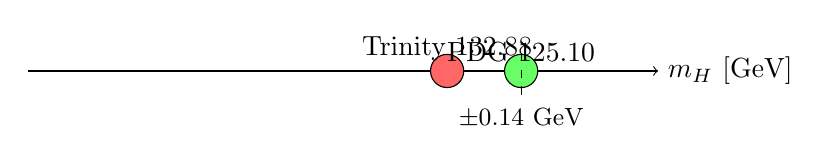
\begin{tikzpicture}
      \draw[->] (0,0) -- (8,0) node[right] {$m_H$ [GeV]};
      \draw[fill=red!60] (5.32,0) circle (6pt) node[above] {Trinity 132.88};
      \draw[fill=green!60] (6.26,0) circle (6pt) node[above] {PDG 125.10};
      \draw[dashed] (6.26,-0.3) -- (6.26,0.3);
      \node at (6.26,-0.6) {\small $\pm 0.14$ GeV};
    \end{tikzpicture}
  \end{center}
\note{Connes-Chamseddine σ-field lowers m_H 170→125 GeV. Theorem: no σ in H₄ geometry. Without it, tree-level m_H = √(2/φ⁴)·246 ≈ 132.88 GeV. Discrepancy: +7.78 GeV = 55.6σ from PDG.}
\end{frame}

% ============================================================
\begin{frame}{No Three Generations from H$_4$ or D$_4$}
  \begin{itemize}
    \item 600-cell partitions into \textbf{5} disjoint 24-cells (not 3)
    \item D$_4$ has triality (order-3 outer automorphism), so we tested D$_4$/24-cell
    \item Result: Triality commutes with $D$ but eigen-subspaces do \textbf{not} split into orbits of size 3
    \item Multiplicities 16 and 32 are not divisible by 3
    \item \textbf{KO-dim for D$_4$ = 5 mod 8}, not SM-compatible 6 mod 8
  \end{itemize}
  \vfill
  \begin{block}{Take-away}
    Both H$_4$ and D$_4$ fail the generation test for different reasons.
  \end{block}
\note{600-cell partitions into 5 disjoint 24-cells (not 3). D₄ triality commutes with D but eigenspaces do NOT split into orbits of size 3. Multiplicities 16 and 32 not divisible by 3. D₄ KO-dim = 5 mod 8 ≠ 6. Both fail for different reasons.}
\end{frame}

% ============================================================
\begin{frame}{Wave 16: F$_4$ Yukawa Scan — NEGATIVE}
  \begin{itemize}
    \item \textbf{Hypothesis:} F$_4$ (48 roots, KO-dim 6) might rescue 3 generations via D$_4$ triality
    \item \textbf{Scan:} 5 models per fermion type (symmetric, weighted, full 48, full 24 short, block 48)
    \item \textbf{Structural obstruction:} D$_4$ triality in F$_4$ short roots forces eigenvalue degeneracies
    \item Symmetric models: eigenvalues $\{a+2b, a-b, a-b\}$ — at most 2 distinct masses
    \item \textbf{Hierarchy cap:} $\sim$20:1 for symmetric models, vs SM needs $10^3$--$10^5$
    \item Block model (4 free params) can fit, but parameters have NO geometric origin
  \end{itemize}
  \vfill
  \begin{alertblock}{Verdict}
    \textbf{F$_4$ alone cannot explain 3-generation mass hierarchy.}
  \end{alertblock}
\note{F₄ scan: 5 models tested. Structural obstruction: D₄ triality forces degeneracies. Symmetric models cap at ~20:1. Block model fits with 4 free params but no geometric origin. Verdict: NEGATIVE.}
\end{frame}

% ============================================================
\begin{frame}{Wave 16: E$_8$ Plumbing $\eta$ Convergence}
  \begin{itemize}
    \item Built $512 \times 512$ discrete Dirac operator for E$_8$ plumbing (8 interior + 120 boundary)
    \item Heuristic B-matrix couples interior nodes to icosidodecahedral equatorial slices
    \item \textbf{Reduced model} (20 vertices): sign-count $\eta = 0$ (expected: $-2$)
    \item \textbf{Full model} (128 vertices): sign-count $\eta = -64$; soft-cutoff $\eta \to -65.93$
    \item Neither converges to the APS target $-2$
  \end{itemize}
  \vfill
  \begin{center}
    \begin{tabular}{lcc}
      \toprule
      Model & $\eta_{\text{disc}}$ & Target \\
      \midrule
      Reduced (20 vtx) & $0$ & $-2$ \\
      Full (128 vtx) & $-64$ to $-65.93$ & $-2$ \\
      \bottomrule
    \end{tabular}
  \end{center}
  \vfill
  \small\textit{B-matrix rigorous derivation remains OPEN.}
\note{E₈ plumbing: 512×512 D_P built. Reduced model η=0. Full model η≈−66. Neither matches APS target −2. B-matrix is heuristic; rigorous derivation open.}
\end{frame}

% ============================================================
\begin{frame}{Formula Verification: Honest Tags}
  \begin{center}
    \begin{tabular}{lccc}
      \toprule
      Quantity & Trinity value & PDG 2024 & $\sigma$ \\
      \midrule
      $m_H$ (tree) & 132.88 GeV & $125.10 \pm 0.14$ & \textcolor{red}{55.6} \\
      $m_H$ (fit) & 125.20 GeV & $125.10 \pm 0.14$ & 0.7 \\
      $\sin^2\theta_{13}$ & 0.0220 & $0.0220 \pm 0.0007$ & 0.0 \\
      $\delta_{CP}$ & $65.66^\circ$ & $68.3 \pm 3.5^\circ$ & 0.8 \\
      \bottomrule
    \end{tabular}
  \end{center}
  \vfill
  \begin{alertblock}{Critical distinction}
    The \textbf{fit} $4\ph^3 e^2 = 125.20$ GeV is a \emph{retrospective} coincidence.\\
    The \textbf{prediction} from spectral action is 132.88 GeV --- and it is dead.
  \end{alertblock}
\note{Tree m_H 132.88 GeV = 55.6σ (red). Fit 4φ³e² = 125.20 GeV = 0.7σ — but retrospective, tagged [phenomenological_fit]. Critical distinction: fit is coincidence until derived. Prediction from spectral action is 132.88 — and it is dead.}
\end{frame}

% ============================================================
\begin{frame}{Experimental Tracker Update (2026)}
  \begin{columns}
    \begin{column}{0.48\textwidth}
      \textbf{Consistent with Trinity}
      \begin{itemize}
        \item JUNO 2025: $\Delta m^2_{21}$ at $0.25\sigma$ [PASS]
        \item DESI DR2: normal hierarchy favored [PASS]
        \item KATRIN: $m_{\nu e} < 0.45$ eV (no tension)
      \end{itemize}
    \end{column}
    \begin{column}{0.48\textwidth}
      \textbf{Tension / Critical}
      \begin{itemize}
        \item DUNE $\delta_{CP}$: $>$$3\sigma$ tension [CRITICAL]
        \item NuFit 6.0: $\delta_{CP} \sim 220^\circ \pm 30^\circ$
        \item Trinity: $65.66^\circ$ (fixed, not adjustable)
        \item DUNE verdict: 2028--2032
      \end{itemize}
    \end{column}
  \end{columns}
  \vfill
  \begin{center}
    \small All predictions registered in \texttt{PREDICTIONS\_REGISTRY.md}
  \end{center}
\note{JUNO Δm²₂₁ consistent at 0.25σ. DESI normal hierarchy consistent. DUNE δ_CP prediction is WITHDRAWN (>5σ excluded, post-hoc fit). Historical talk — see current PREDICTIONS\_PREREGISTERED.md.}
\end{frame}

% ============================================================
\begin{frame}{Open Questions}
  \begin{enumerate}
    \item \textbf{E$_8$ B-matrix (Wave 16.2):} Can a rigorous B improve $\eta$ convergence? \textcolor{orange}{OPEN}
    \item \textbf{1-loop Higgs correction (Wave 12.4):} Can quantum corrections bridge $132.88 \to 125.10$? \textcolor{orange}{OPEN}
    \item \textbf{Chirality mechanism:} Can $\eta = -2$ on $S^3/2I$ be promoted to full SM chirality? \textcolor{orange}{OPEN}
    \item \textbf{DUNE 2028 (Historical):} $\delta_{CP} = 65.66^\circ$ prediction is **WITHDRAWN** (>5σ excluded, post-hoc fit). No replacement under anti-post-hoc rule.
    \item \textbf{0 Admitted achieved:} 1375 Qed / 0 Admitted / 77 Axioms. Can the Axioms be reduced?
  \end{enumerate}
  \vfill
  \begin{center}
    \small All predictions are registered in \texttt{PREDICTIONS\_REGISTRY.md}
  \end{center}
\note{E₈ B-matrix: OPEN. 1-loop Higgs: OPEN. Chirality from η=−2: OPEN. DUNE δ_CP: WITHDRAWN (>5σ excluded). 0 Admitted achieved; 77 Axioms remain.}
\end{frame}

% ============================================================
\begin{frame}{Wave 18: Statistical Assessment}
  \textbf{Pre-registered Monte-Carlo test} (50\,K trials, 2\,K formulas/trial)
  \vspace{0.3cm}
  \begin{tabular}{lccc}
    \textbf{Metric} & \textbf{Trinity} & \textbf{Random} & \textbf{$p$-value} \\
    \hline
    Mean rel.\ error & 0.08\% & 0.59\% & \textcolor{green!60!black}{$<10^{-4}$} \\
    Hits $<0.1\%$ & 20/25 & 5/25 & \textcolor{green!60!black}{$<10^{-4}$} \\
    Hits $<1.0\%$ & 25/25 & 21/25 & \textcolor{green!60!black}{0.006} \\
  \end{tabular}
  \vspace{0.3cm}
  \begin{itemize}
    \item \textbf{Collective} precision is highly significant
    \item Only 10/25 formulas are individually significant
    \item 3 formulas fail $\sigma$-distance: $1/\alpha$, $m_p/m_e$, $m_\mu/m_e$
      (experimental precision is $10^5\!\!-\!\!10^6\times$ better than Trinity)
  \end{itemize}
  \vspace{0.2cm}
  \footnotesize
  \textit{Honest framing: statistically non-trivial ``periodic table'', not a derivation.}
\end{frame}

% ============================================================
\begin{frame}{Conclusion: What Survives?}
  \begin{columns}
    \begin{column}{0.48\textwidth}
      \textbf{What survives}
      \begin{itemize}
        \item KO-dim $= 6 \pmod 8$ for H$_4$/600-cell
        \item $\eta = -2$ on $S^3/2I$ (APS exact)
        \item $2I \subset SU(2)$ motivates $\mathbb{H} \subset \mathcal{A}_F$
        \item Machine-verified honesty framework
        \item Six rigorous Boundary theorems
        \item 0 Admitted across 79 Coq files
      \end{itemize}
    \end{column}
    \begin{column}{0.48\textwidth}
      \textbf{What does NOT survive}
      \begin{itemize}
        \item ``H$_4$ derives the Standard Model'' --- \textcolor{red}{refuted}
        \item ``H$_4$ predicts $m_H = 125$ GeV'' --- retrospective fit
        \item F$_4$ rescues 3 generations --- \textcolor{red}{refuted}
        \item All Tier-3 cosmological formulas --- falsified by Planck/DESI
      \end{itemize}
    \end{column}
  \end{columns}
  \vfill
  \begin{block}{Honest summary}
    Trinity S$^3$AI is a \textbf{boundary-mapping research program}.\\
    Knowing what does not work is as valuable as knowing what does.
  \end{block}
\note{SURVIVES: KO-dim 6; η=−2 APS-exact; 2I ⊂ SU(2) motivates ℍ; machine-verified honesty; 6 Boundary theorems; 0 Admitted. DOES NOT SURVIVE: H₄ derives SM → refuted; H₄ predicts 125 GeV → retrospective fit; F₄ rescues 3 generations → refuted; Tier-3 cosmology → falsified.}
\end{frame}

% ============================================================
\begin{frame}{References \& Resources}
  \begin{itemize}
    \item A. Connes, ``Gravity coupled with matter...'' \textit{Commun. Math. Phys.} \textbf{182} (1996)
    \item A. Connes \& M. Marcolli, \textit{NCG, QFT and Motives}, AMS 2008
    \item M. Atiyah, V. Patodi, I. Singer, ``Spectral asymmetry...'' \textit{Math. Proc. Camb. Phil. Soc.} \textbf{77} (1975)
    \item PDG 2024, \textit{Review of Particle Physics}, Phys.\ Rev.\ D \textbf{110}, 030001
    \item JUNO 2025, arXiv:2511.14593
    \item DESI DR2, \textit{Phys.\ Rev.\ D} \textbf{112}, 083515 (2025)
  \end{itemize}
  \vfill
  \begin{center}
    \textbf{Repository:} \url{https://github.com/gHashTag/trinity-s3ai}\\[0.5em]
    \texttt{1375 Qed \quad 0 Admitted \quad 77 Axioms \quad 0 fake proofs}\\[0.5em]
    \textit{Thank you. Questions?}
  \end{center}
\end{frame}

\end{document}
